\documentclass[conference]{IEEEtran}
\IEEEoverridecommandlockouts

% --- Packages ---
\usepackage{cite}
\usepackage{amsmath,amssymb,amsfonts}
\usepackage{amsthm}
\usepackage{algorithm}
\usepackage{algorithmic}
\usepackage{graphicx}
\usepackage{textcomp}
\usepackage{xcolor}
\usepackage{booktabs}
\usepackage{multirow}
\usepackage{array}
\usepackage[hidelinks]{hyperref}

\newtheorem{theorem}{Theorem}
\newtheorem{lemma}{Lemma}
\newtheorem{proposition}{Proposition}
\newtheorem{definition}{Definition}
\newtheorem{assumption}{Assumption}

\newcommand{\PH}[1]{{\color{red}\textbf{[#1]}}}

\begin{document}

\title{\LARGE \bf
The Topological Cage: Search-Free Geometric Injection and \\
Multi-Homotopy Routing on a Bounded Medial Manifold
}

\author{Shubham Puri Goswami$^{1}$ and Ravi Prakash$^{2}$%
\thanks{$^{1}$Shubham Puri Goswami is with the Department of Cyber Physical Systems, Indian Institute of Science, Bengaluru, India {\tt\small shubhampg@iisc.ac.in}}%
\thanks{$^{2}$Ravi Prakash is with the Department of Cyber Physical Systems, Indian Institute of Science, Bengaluru, India {\tt\small ravipr@iisc.ac.in}}%
}

\maketitle
\thispagestyle{empty}
\pagestyle{empty}

% ==========================================
% ABSTRACT
% ==========================================
\begin{abstract}
Medial-axis and generalized Voronoi representations give mobile robots a compact, maximum-clearance backbone of free space, but two structural defects block their use as a standalone planning layer. First, the \emph{injection problem}: an arbitrary start or goal does not lie on the skeleton, and connecting it back is usually done with the same grid search the skeleton was meant to replace. Second, the \emph{Voronoi void}: because the medial axis requires equidistance to two or more obstacle boundaries, wide open regions and free-standing obstacle islands produce sparse or disconnected components, so the routing graph is not globally connected.

We propose the \emph{Topological Cage}, a purely geometric construction that closes the medial axis into a bounded manifold. Free space is represented by a Euclidean distance field; the medial ridge is pruned by a tangent--gradient parallelism test that retains structured interior and inter-island corridors while removing unbounded exterior branches; the pruned skeleton is then unioned with a single distance level set placed above the interior clearance supremum. Start and goal are attached by integrating the normalized distance gradient in both directions, which terminates in finite arc length without graph expansion. Routing reduces to a search on a sparse graph whose size depends on environment topology rather than map area, and the released budget is spent enumerating homotopy classes, selected by a lexicographic bottleneck order on sorted clearance profiles. The selected class is smoothed by a damped spring--mass band with per-obstacle selective clearance relaxation, distributed decimation, and a kinetic-energy stopping rule. Across four benchmark environments, $400$ randomized queries and three operator-drawn complex maps, closure reduces routing-structure components from $21$ to $5$ and raises query feasibility from $24.0\%$ to $99.6\%$ of attainable; gradient injection attaches terminals with $100\%$ success and zero connector collisions using $58.9$ integration steps against $44{,}345$ cell expansions for grid search; the lexicographic criterion cuts selection ties by $56.7\%$ while raising mean clearance; and the damped band reduces integrated curvature by $85.2\%$ and node-spacing dispersion by $97.4\%$.
\end{abstract}

% ==========================================
% I. INTRODUCTION
% ==========================================
\section{Introduction}

Mobile robots operating in cluttered indoor environments must repeatedly answer start-to-goal queries on a map that is largely static. Grid search (A$^\star$, Dijkstra) is resolution-complete but expands a number of cells that grows with the free area, and because it minimizes path length it produces trajectories that hug obstacle boundaries unless an inflation layer is tuned by hand. Sampling planners (PRM, RRT$^\star$) scale better in dimension, but narrow doorways and non-convex traps require sampling densities that erode their advantage.

Distance-field skeletons take the opposite approach: they precompute the locus of maximum clearance once, and route on it. This gives clearance by construction and a graph orders of magnitude smaller than the grid~\cite{lau2013,oleynikova2018,qi2022pruned}. Recent work has made this representation practical online, including incremental updates~\cite{lau2013} and, closest to our setting, the Enveloped Generalized Voronoi Graph (EGVG)~\cite{qi2025egvg}, which augments the Voronoi skeleton with distance-field contour bands.

Two problems remain, and they are the subject of this paper.

\textbf{The injection problem.} A query point almost never lies on the skeleton. Nearest-pixel projection is brittle and can cut through obstacles; inserting the query as a temporary obstacle forces a local skeleton rebuild; running A$^\star$ or BFS from the query until a skeleton pixel is hit reintroduces grid expansion, and its cost grows with the distance to the skeleton, which is exactly the open-space case that is most common~\cite{qi2025egvg,oleynikova2018}. Raycasting toward nearby vertices~\cite{qi2025egvg} is fast but is not guaranteed to succeed, and its success rate depends on vertex placement. Our measurements confirm both failure modes: nearest-pixel projection produces a colliding connector on $2.1\%$ of terminals, and raycast injection fails on $6.5\%$ of terminals in the non-convex environment (Table~\ref{tab:injection}).

\textbf{The Voronoi void.} The medial axis is defined by equidistance to two or more boundaries. In an expansive room, or around a free-standing obstacle island, the resulting branches are sparse, or form a component disconnected from the rest of the graph. Measured over our four benchmarks, the raw pruned skeleton splits into $21$ components and the resulting planner declares only $24.0\%$ of randomized queries feasible, despite the free space admitting a solution for $93.0\%$ of them.

Both defects share a root cause: the skeleton is an \emph{open, possibly disconnected} set, while the query can be anywhere in free space. Our response is to make the routing structure \emph{closed and connected by construction}. We prune the raw medial axis to its structured interior, take the clearance supremum $C_{\max}$ over that interior, and add the distance level set at $C_{\max}+\Delta$. Because the level set sits above every interior clearance value, it encloses the interior structure, and its union with the pruned skeleton is a bounded manifold --- the \emph{Topological Cage}. Gradient ascent from any free point either reaches a ridge (in the cage) or crosses the level set (in the cage), so injection succeeds without search.

This changes the cost structure of the planner. Map processing is paid once; each query costs a bounded number of gradient steps plus a search on a graph whose size depends on environment topology rather than map area. The residual budget buys what per-query grid planners cannot afford: enumerating $K$ topologically distinct routes and selecting among them by clearance rather than length.

\textbf{Contributions.}
\begin{itemize}
  \item A bounded medial manifold (the Topological Cage) built from a tangent--gradient pruning rule and a single super-critical distance level set, which unifies disconnected skeleton components and isolated obstacle islands into one routing graph, raising query feasibility from $24.0\%$ to $99.6\%$ of attainable (Sec.~\ref{sec:offline}).
  \item A search-free bidirectional gradient injection procedure with a finite-termination guarantee, achieving $100\%$ attachment success and zero connector collisions at $58.9$ integration steps per terminal, against $2{,}443$ expansions for the A$^\star$ fallback (Sec.~\ref{sec:online}).
  \item A lexicographic bottleneck criterion over sorted clearance profiles that strictly refines min-clearance selection, cutting selection ties by $56.7\%$ while raising mean path clearance (Sec.~\ref{sec:opt}).
  \item A damped spring--mass band with per-obstacle selective clearance relaxation, distributed decimation, and a kinetic-energy stopping rule, reducing integrated curvature by $85.2\%$ and node-spacing dispersion by $97.4\%$ relative to the raw skeletal route (Sec.~\ref{sec:opt}).
\end{itemize}

% ==========================================
% II. RELATED WORK
% ==========================================
\section{Related Work}

\textbf{Search and sampling planners.} A$^\star$~\cite{hart1968} and its replanning variants~\cite{koenig2005} are resolution-complete but expand cells proportional to explored free area, and are length-optimal rather than clearance-optimal. PRM~\cite{kavraki1996} amortizes construction across queries, which is the correct instinct, but uniform sampling under-represents narrow passages, so the density needed to capture doorways inflates both memory and construction cost. RRT$^\star$~\cite{karaman2011,lavalle1998} converges to optimality asymptotically but is not naturally multi-query. Visibility graphs~\cite{yang2022far} and sparse roadmaps~\cite{dobson2014} reduce graph size but grow with explored area.

\textbf{Skeleton and Voronoi representations.} GVD/GVG methods extract the ridge set of the distance field~\cite{lau2013,hoff1999}. They are compact and clearance-maximal, and have been used as heuristics for RRT~\cite{chi2022}, for AGV two-layer planning~\cite{zhang2024agv}, and for aerial topological graphs~\cite{oleynikova2018}. Skeleton simplification by angle criteria was introduced by Foskey et al.~\cite{foskey2003}; we use a related but distinct test, applied between the skeleton tangent and the distance gradient, to separate bounded interior corridors from unbounded exterior branches. EGVG~\cite{qi2025egvg} is the closest representation to ours: it also adds distance-field contours to the skeleton. The difference is purpose and placement. EGVG adds contour bands \emph{around obstacles} at a user-chosen $d_c$ to increase spatial expressiveness, and still connects terminals by raycasting to nearby vertices. We add \emph{one} contour at a level above the interior clearance supremum, whose role is topological closure rather than expressiveness, and we use that closure to obtain a terminal-connection procedure needing no raycast, no temporary obstacle insertion, and no local search.

\textbf{Local optimization.} DWA~\cite{fox1997} and TEB~\cite{rosmann2012} are the deployed standard. Elastic bands~\cite{quinlan1993} smooth a global path by balancing internal contraction against obstacle repulsion. Two known failure modes motivate our variant: in tight corridors the repulsion term can dominate contraction and cause oscillation or freezing, and nodes with no enforced rest length slide along the path and clump. We address the first with per-obstacle relaxation of the repulsion threshold on exactly the walls the selected route must squeeze past, and the second with a Hookean rest length plus uniformly distributed decimation.

\textbf{Multi-homotopy selection.} Enumerating homotopy classes and choosing among them is established~\cite{bhattacharya2012,qi2025egvg}. EGVG enumerates by progressive vertex suppression and selects by a weighted cost of length, heading deviation, and deviation from the previous path~\cite{qi2025egvg}. We enumerate by $K$-shortest paths~\cite{yen1971} over the cage graph and select by a clearance-lexicographic order, optimizing safety first and using geometric cost only as a subsequent tiebreak.

% ==========================================
% III. PROBLEM FORMULATION
% ==========================================
\section{Problem Formulation}
\label{sec:problem}

\subsection{Setting and Notation}

Let $\mathcal{W}\subset\mathbb{R}^2$ be a bounded workspace discretized on a grid with resolution $r$ (m/pixel). Let $\mathcal{O}\subset\mathcal{W}$ denote the closed obstacle set and $\Omega=\mathcal{W}\setminus\mathcal{O}$ the open free set. The robot is a disc of radius $\rho$ with differential-drive kinematics; planning is performed in $\mathbb{R}^2$ and the resulting path is tracked by a local controller. Notation is collected in Table~\ref{tab:notation}.

\begin{table}[htbp]
\caption{Notation}
\label{tab:notation}
\begin{center}
\renewcommand{\arraystretch}{1.12}
\begin{tabular}{@{}ll@{}}
\toprule
\textbf{Symbol} & \textbf{Meaning} \\ \midrule
$\Omega,\ \mathcal{O}$ & free space, obstacle set \\
$\Psi(p)$ & Euclidean distance from $p\in\Omega$ to $\partial\mathcal{O}$ \\
$\nabla\Psi(p)$ & spatial gradient of $\Psi$; unit form $\hat{n}(p)$ \\
$\mathcal{M}$ & raw medial ridge set of $\Psi$ \\
$\hat{t}_{\mathcal{M}}(p)$ & unit tangent of $\mathcal{M}$ at $p$ \\
$\tau$ & angular tolerance of the parallelism test \\
$\mathcal{M}_{\mathrm{int}}$ & interior (structured) subset of $\mathcal{M}$ \\
$C_{\max}$ & clearance supremum over $\mathcal{M}_{\mathrm{int}}$ \\
$\Delta$ & cage offset above $C_{\max}$ \\
$d_{\mathrm{cage}}$ & $C_{\max}+\Delta$, cage level-set value \\
$\mathcal{B}$ & level set $\{\Psi = d_{\mathrm{cage}}\}$ \\
$\mathcal{C}$ & Topological Cage, $\mathcal{M}_{\mathrm{trim}}\cup\mathcal{B}$ \\
$G=(V,E)$ & sparse graph abstracted from $\mathcal{C}$ \\
$p_S,p_G$ & query start and goal in $\Omega$ \\
$p_S',p_G'$ & their injection points on $\mathcal{C}$ \\
$\alpha$ & gradient integration step (pixels) \\
$K$ & number of enumerated homotopy candidates \\
$\sigma(P)$ & ascending-sorted clearance profile of path $P$ \\
$P_i$ & $i$-th band node; $d_{\mathrm{rest}}$ its rest spacing \\
$\tau_O$ & repulsion threshold for obstacle component $O$ \\
$W_s,W_r,D$ & spring, repulsion, damping coefficients \\
$\epsilon_{\mathrm{stab}}$ & velocity threshold for auto-stop \\
$\rho+\delta_{\mathrm{safe}}$ & hard safety floor \\ \bottomrule
\end{tabular}
\end{center}
\end{table}

\begin{assumption}
The map is static during a query batch, $\partial\mathcal{O}$ is known, and $\Omega$ is bounded. $\Psi$ is computed by an exact Euclidean distance transform~\cite{felzenszwalb2012} and is therefore $1$-Lipschitz on $\Omega$.
\end{assumption}

\subsection{The Problems Addressed}

\textbf{(P1) Terminal injection without search.} Given $p_S,p_G\in\Omega$ with $p_S,p_G\notin\mathcal{M}$, construct collision-free connections onto the routing structure whose cost does not scale with $|\Omega|$ and whose success is guaranteed rather than empirical. This is difficult because $\mathcal{M}$ is a measure-zero set: geometric projection is unsafe, and completeness-preserving alternatives are searches. Evidence required: injection success rate over randomized terminals, connector collision rate, and cost against a BFS/A$^\star$ fallback. Reported in Table~\ref{tab:injection}.

\textbf{(P2) Global connectivity of the routing structure.} Given that $\mathcal{M}$ may consist of disjoint components --- sparse branches in open rooms, closed loops around free-standing islands --- construct a connected superset $\mathcal{C}\supseteq\mathcal{M}_{\mathrm{int}}$ without heuristic bridging. Consequence of failure: the planner reports infeasible for a feasible query, as EGVG explicitly does when terminals fall in different subgraphs~\cite{qi2025egvg}. Evidence required: component count before and after closure, and query feasibility rate. Reported in Table~\ref{tab:connectivity}.

\textbf{(P3) Homotopy selection under a clearance objective.} Given $K$ topologically distinct routes, select the safest with a deterministic total order. Minimum clearance alone is a coarse statistic and ties frequently when candidates share a bottleneck corridor. Evidence required: tie frequency and clearance against min-clearance and shortest-length selection. Reported in Table~\ref{tab:clearance}.

\textbf{(P4) Executable smoothing without corridor instability.} Convert the clearance-maximal but jagged skeletal route into a smooth path without triggering repulsion-dominance oscillation or node clumping. Evidence required: node-spacing dispersion, curvature and angular jerk, and settling behaviour. Reported in Table~\ref{tab:kinematics}.

P1 and P2 are the primary problems; they are what make the cage necessary. P3 and P4 are enabled by the budget that P1 and P2 release, and are secondary contributions.

% ==========================================
% IV. OFFLINE CONSTRUCTION
% ==========================================
\section{Offline Construction of the Topological Cage}
\label{sec:offline}

This stage is executed once per static map. Its output is a bounded set $\mathcal{C}$ and a sparse graph $G$.

\subsection{Distance Field}

We compute the exact Euclidean distance transform of $\Omega$~\cite{felzenszwalb2012},
\begin{equation}
\Psi(p)=\min_{q\in\partial\mathcal{O}}\|p-q\|_2,\qquad p\in\Omega ,
\end{equation}
and its gradient by central differences,
\begin{equation}
\nabla\Psi(p)=\Big[\tfrac{\Psi(p+e_x)-\Psi(p-e_x)}{2},\ \tfrac{\Psi(p+e_y)-\Psi(p-e_y)}{2}\Big]^{\!\top},
\end{equation}
with $\hat{n}(p)=\nabla\Psi(p)/\|\nabla\Psi(p)\|$ wherever $\|\nabla\Psi(p)\|>0$. $\Psi$ is $1$-Lipschitz and differentiable everywhere except on $\mathcal{M}$, where the nearest-boundary point is non-unique. $\hat{n}$ points away from the nearest obstacle, so following $+\hat{n}$ increases clearance monotonically (Fig.~\ref{fig:scalar_field}).

\begin{figure}[htbp]
\centerline{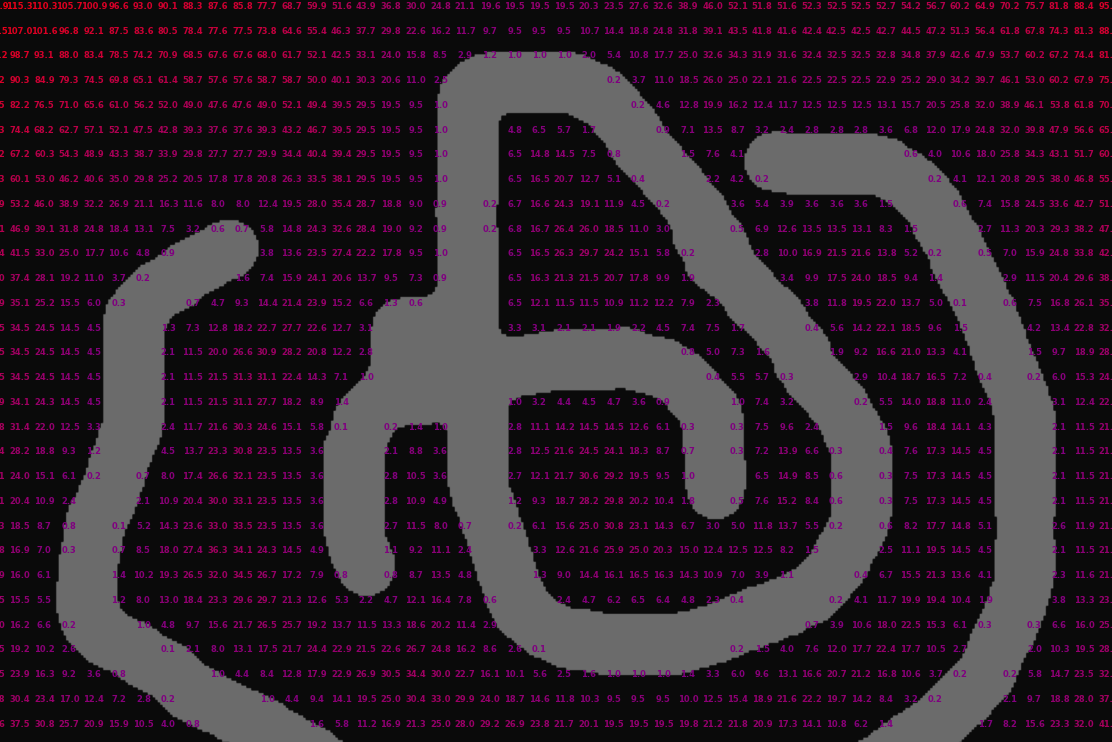
\includegraphics[width=0.92\columnwidth]{5.png}}
\caption{Discretized distance field. Cell values are the exact Euclidean distance $\Psi$ to the nearest obstacle; the induced gradient field $\nabla\Psi$ (arrows) is the vector field along which terminal injection is integrated. \emph{Reader takeaway: the entire free space carries a defined direction of increasing clearance, which is what makes search-free injection possible.}}
\label{fig:scalar_field}
\end{figure}

\subsection{Medial Ridge Extraction}

The raw medial set is the ridge of $\Psi$, i.e.\ points where gradient directions from opposing boundaries meet:
\begin{equation}
\mathcal{M}=\{p\in\Omega \mid \exists\, p_i,p_j\in N(p):\ \nabla\Psi(p_i)\cdot\nabla\Psi(p_j)<0\},
\label{eq:ridge}
\end{equation}
with $N(p)$ the $8$-neighborhood. Eq.~\eqref{eq:ridge} is the standard ridge criterion and is not claimed as a contribution; it is stated because both pruning and closure operate on its output. $\mathcal{M}$ is thinned to one-pixel width.

$\mathcal{M}$ has two defects, visible in Fig.~\ref{fig:raw_medial_axis}. It emits unbounded branches into open space, so it is not a bounded set; and in wide regions and around free-standing islands it is sparse or splits into components with no connection to the main structure. Measured component counts appear in Table~\ref{tab:connectivity}.

\begin{figure}[htbp]
\centerline{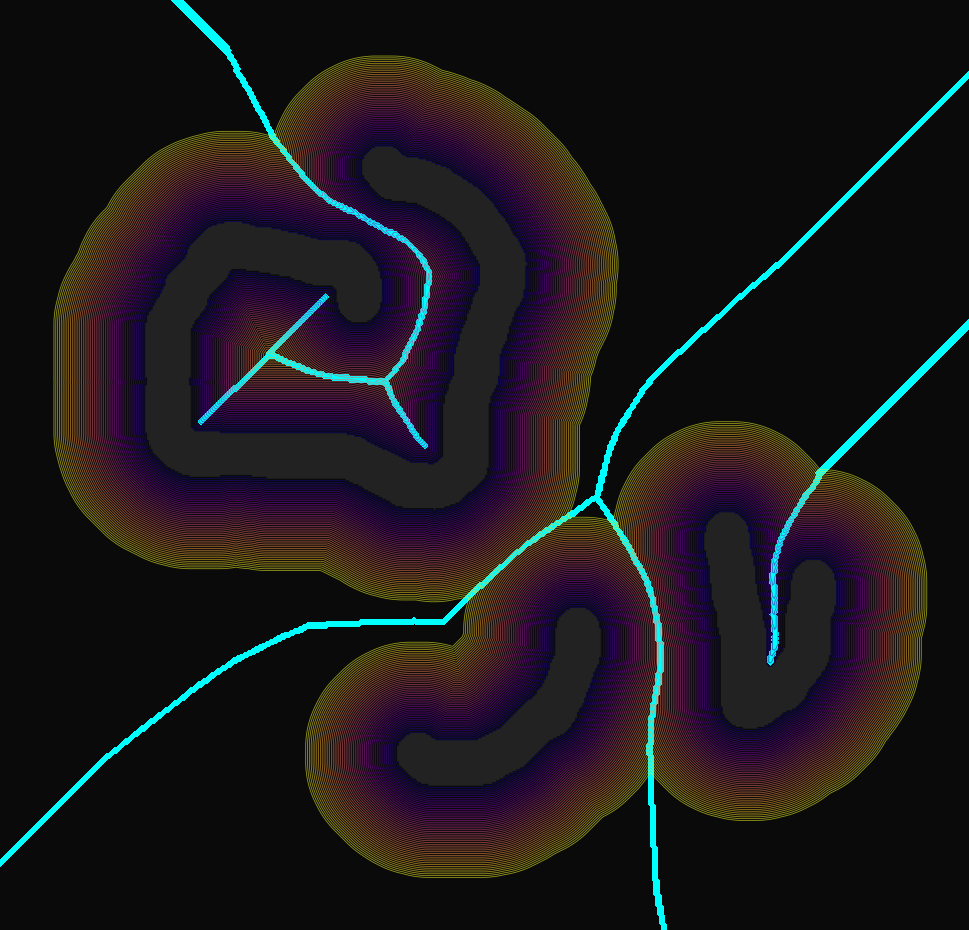
\includegraphics[width=\columnwidth]{infinitemedial.png}}
\caption{Raw medial ridge (cyan) extracted from the distance field. Interior corridors between obstacles are captured correctly, but branches protrude into open space without terminating, and the structure around isolated obstacles forms components that do not connect to the main skeleton. \emph{Reader takeaway: the raw skeleton is neither bounded nor connected, so it cannot serve as a routing structure on its own.}}
\label{fig:raw_medial_axis}
\end{figure}

\subsection{Tangent--Gradient Pruning}

We separate structured interior corridors from unbounded exterior branches with a local geometric test. Inside a corridor the medial curve runs parallel to the flanking walls, so the distance gradient is close to orthogonal to the skeleton tangent. On an exterior branch radiating into open space, this orthogonality breaks down. Let $\hat{t}_{\mathcal{M}}(p)$ be the unit tangent of $\mathcal{M}$ at $p$, estimated by principal direction over a local window of skeleton pixels, and let $\theta(p)$ be the deviation from orthogonality:
\begin{equation}
\theta(p)=\Big|\,90^\circ-\arccos\big|\hat{t}_{\mathcal{M}}(p)\cdot \hat{n}(p)\big|\,\Big| .
\end{equation}
The interior subset is
\begin{equation}
\mathcal{M}_{\mathrm{int}}=\big\{p\in\mathcal{M}\ \big|\ \big|\hat{t}_{\mathcal{M}}(p)\cdot\hat{n}(p)\big|\le \cos(90^\circ-\tau)\big\},
\label{eq:prune}
\end{equation}
with angular tolerance $\tau$; Eq.~\eqref{eq:prune} keeps $p$ when $\theta(p)\le\tau$. The projection $|\hat{t}_{\mathcal{M}}\cdot\nabla\Psi|$ is evaluated as the directional derivative of $\Psi$ taken along $\hat{t}_{\mathcal{M}}$, which is well defined on the ridge itself where $\nabla\Psi$ is not.

Two properties matter. First, the test is local and needs no connectivity analysis, so it costs $O(|\mathcal{M}|)$. Second, the medial curve forming \emph{between two separate obstacle islands} also satisfies the parallelism condition, because locally it is still a corridor. The same threshold therefore preserves inter-island connectivity while discarding exterior rays, which is what allows a single scalar $\tau$ to handle both continuous-wall and island topologies. Fig.~\ref{fig:angle_cutoff} shows representative angles on each class of branch. We use $\tau=17^\circ$; the sweep in Sec.~\ref{sec:ablation} shows feasibility is invariant over $\tau\in[8^\circ,45^\circ]$, so the specific value is not load-bearing.

The retained set is trimmed of residual stubs shorter than $\ell_{\min}$ pixels, giving $\mathcal{M}_{\mathrm{trim}}$.

\begin{figure}[htbp]
\centerline{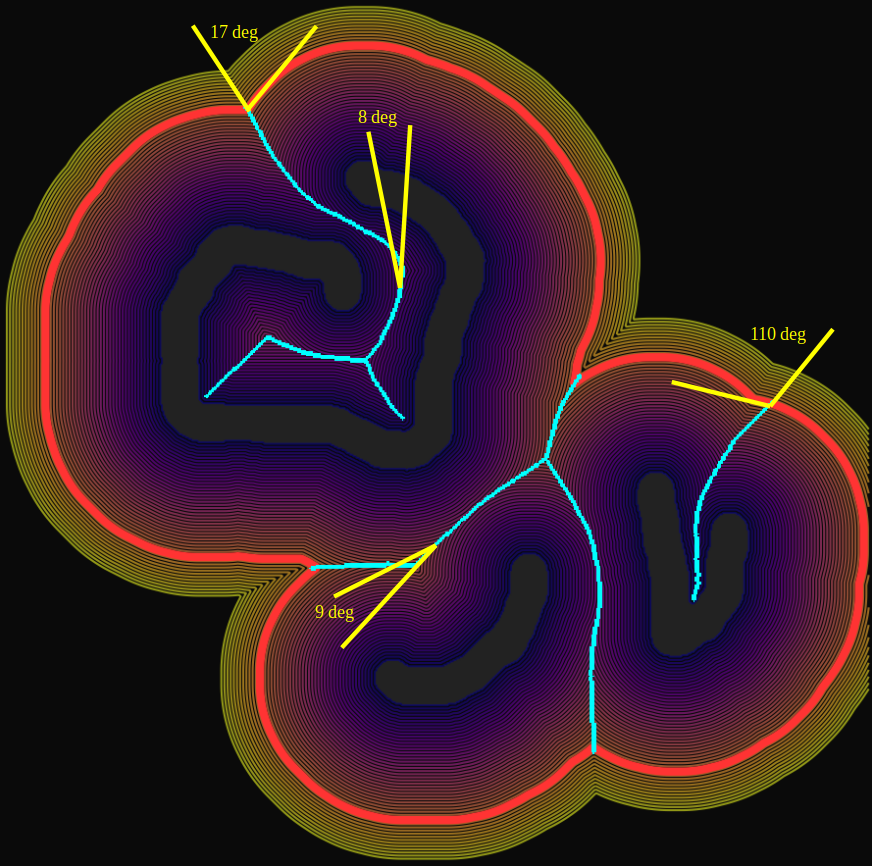
\includegraphics[width=\columnwidth]{angleprunning.png}}
\caption{Tangent--gradient pruning across wall and island topologies. Interior corridors show near-orthogonal tangent/gradient pairs ($\theta\!\approx\!8^\circ$), exterior branches diverge strongly ($\theta\!\approx\!110^\circ$) and are removed, and the corridor formed between two free-standing islands remains parallel ($\theta\!\approx\!9^\circ$) and is retained by the same $\tau=17^\circ$ threshold. \emph{Reader takeaway: one local angular test distinguishes bounded interior structure from unbounded exterior structure, without a global connectivity pass.}}
\label{fig:angle_cutoff}
\end{figure}

\subsection{Closure by a Super-Critical Level Set}

Let
\begin{equation}
C_{\max}=\sup_{p\in\mathcal{M}_{\mathrm{int}}}\Psi(p),
\end{equation}
the clearance radius of the widest \emph{interior} corridor. Choose an offset $\Delta>0$ and set $d_{\mathrm{cage}}=C_{\max}+\Delta$. Define the discrete level set
\begin{equation}
\mathcal{B}=\{p\in\Omega\ \mid\ |\Psi(p)-d_{\mathrm{cage}}|\le\varepsilon\},
\end{equation}
with $\varepsilon$ half the grid diagonal so $\mathcal{B}$ is one pixel thick after connectivity repair. The level is additionally clamped to the attained range of $\Psi$ on $\Omega$, so that $\mathcal{B}$ is non-empty on maps whose widest interior corridor coincides with the global clearance maximum. The Topological Cage is
\begin{equation}
\boxed{\ \mathcal{C}=\mathcal{M}_{\mathrm{trim}}\ \cup\ \mathcal{B}\ }
\label{eq:cage}
\end{equation}

The role of each term is distinct. $\mathcal{M}_{\mathrm{trim}}$ supplies clearance-maximal corridors where corridors exist. $\mathcal{B}$ supplies a closed envelope where they do not, and simultaneously provides a connection medium between components of $\mathcal{M}_{\mathrm{trim}}$. Because $d_{\mathrm{cage}}>\Psi(p)$ for every $p\in\mathcal{M}_{\mathrm{int}}$, no interior structure lies outside $\mathcal{B}$. Fig.~\ref{fig:semantic_cage} shows the assembled structure over a semantically annotated map in which rigid and deformable obstacle classes carry different clearance thresholds $\tau_O$.

The distinction from EGVG's contour augmentation~\cite{qi2025egvg} is the placement rule. EGVG places bands at a user-chosen $d_c$ near obstacles to enrich representation. We place a single band at a level determined by the map itself, $C_{\max}+\Delta$, because only a super-critical level guarantees enclosure. Consistent with this, the sweep in Sec.~\ref{sec:ablation} finds feasibility invariant over $\Delta\in[5,80]$~px: $\Delta$ controls how far the envelope sits from the interior structure, not whether enclosure holds.

\begin{figure}[htbp]
\centerline{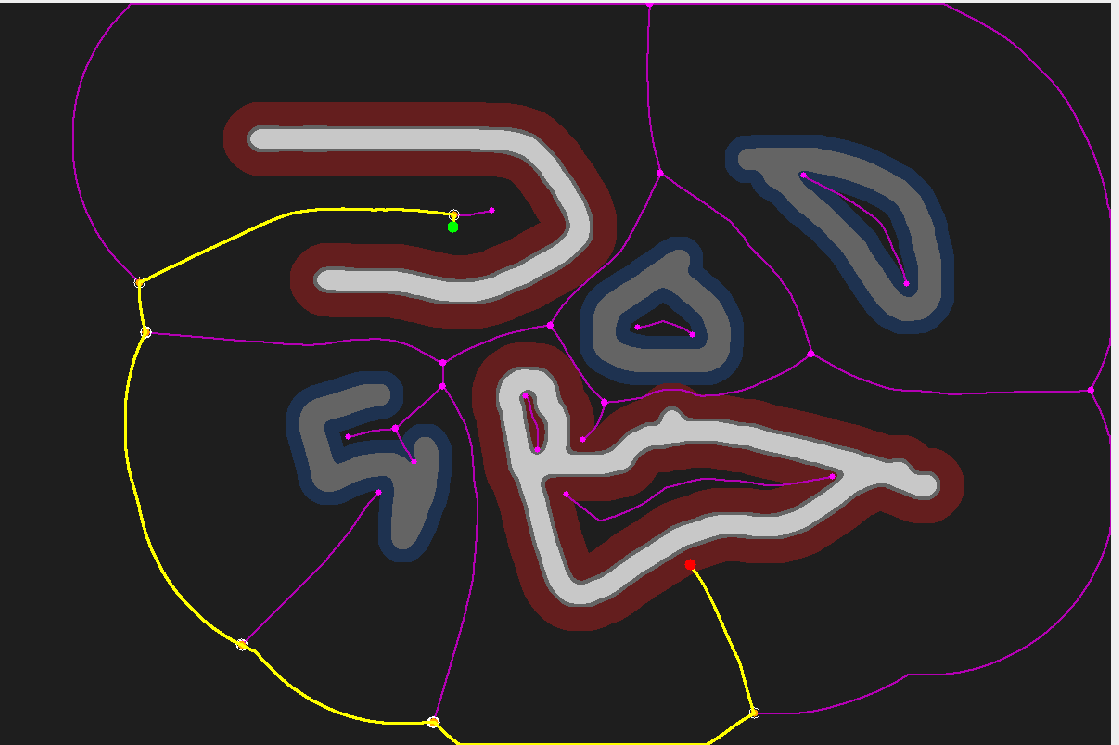
\includegraphics[width=\columnwidth]{medialplusband.png}}
\caption{Assembled Topological Cage (purple) on a semantically annotated map. Rigid (red band) and deformable (blue band) obstacle classes carry different clearance thresholds. The single super-critical level set encloses all interior corridors and all isolated island structures, producing one connected routing manifold; a representative route is shown in yellow. \emph{Reader takeaway: after closure, no free-space region is topologically stranded.}}
\label{fig:semantic_cage}
\end{figure}

\subsection{Graph Abstraction}

$\mathcal{C}$ is compressed to a sparse graph $G=(V,E)$ by pixel-degree classification, following standard practice~\cite{qi2025egvg,lau2013}: pixels of degree $\ge 3$ are junction vertices, degree $1$ are endpoints, degree $2$ are edge interior. Flood-fill along degree-$2$ chains produces edges. Junction vertices within a small radius are clustered to avoid redundant topology. Any pixel with $\Psi(p)<\rho+\delta_{\mathrm{safe}}$ is discarded before abstraction, so every path on $G$ is collision-free by construction and no edge-wise collision checking is needed at query time.

Edge cost is the accumulated axis displacement of the underlying pixel chain $\{p_0,\dots,p_K\}$,
\begin{equation}
g(e)=\sqrt{a_x(e)^2+a_y(e)^2},\quad a_d(e)=\!\!\sum_{k=0}^{K-1}\!\!|d_{k+1}-d_k| ,
\end{equation}
for $d\in\{x,y\}$. Each edge additionally stores its clearance profile $\{\Psi(p_k)\}$, which the selection stage of Sec.~\ref{sec:opt} consumes.

The resulting graphs contain $45$--$115$ vertices and $63$--$161$ edges on $375{,}000$-pixel maps (Table~\ref{tab:breakdown}), i.e.\ a compression of roughly three orders of magnitude, and their size tracks environment topology rather than pixel count.

% ==========================================
% V. ONLINE PHASE
% ==========================================
\section{Online Query: Search-Free Injection}
\label{sec:online}

\subsection{Bidirectional Gradient Scouts}

Given $p_S$ (and identically $p_G$), we integrate the normalized gradient field in both directions,
\begin{equation}
p_{k+1}=p_k \pm \alpha\,\hat{n}(p_k),\qquad p_0=p_S ,
\label{eq:scout}
\end{equation}
terminating when $p_{k+1}$ lies within one pixel of $\mathcal{C}$. The $+$ branch (``climber'') ascends toward higher clearance; the $-$ branch (``diver'') descends toward the nearest boundary. Both attachment points are retained and inserted into $G$ as temporary vertices, and the search runs over the union. The ablation in Sec.~\ref{sec:ablation} quantifies the split: the climber alone attaches $83.8\%$ of terminals, and the bidirectional pair raises this to $94.4\%$.

Step size $\alpha$ trades accuracy against iteration count. Near the ridge $\nabla\Psi$ is discontinuous, so we clamp the step and terminate on cage contact before the discontinuity is reached; the integration need not be exact, only to make contact. The sweep in Sec.~\ref{sec:ablation} shows $100\%$ attachment for $\alpha\in[0.25,2.0]$~px with step counts falling from $127.5$ to $17.2$. Fig.~\ref{fig:scouts} illustrates both branches.

\begin{figure}[htbp]
\centerline{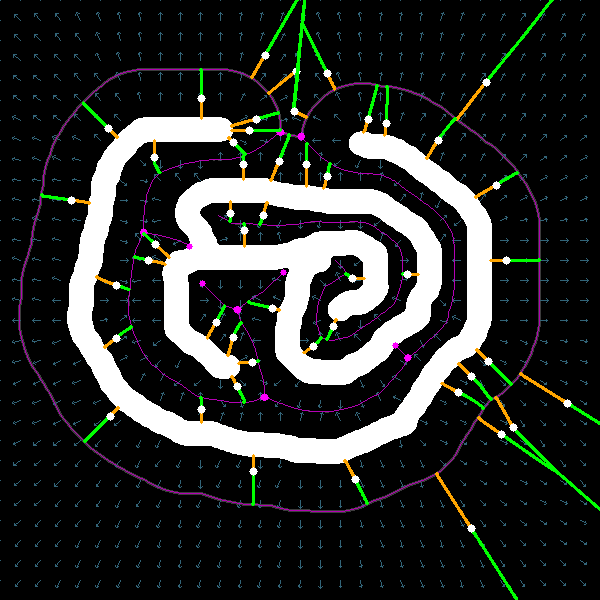
\includegraphics[width=0.85\columnwidth]{scout_navigation_map.png}}
\caption{Search-free terminal injection. From an arbitrary query point, the climber (green) integrates $+\hat{n}$ and the diver (orange) integrates $-\hat{n}$ until either trajectory contacts the cage (purple). Both contact points are inserted into the graph, seeding distinct homotopy classes. \emph{Reader takeaway: connecting a terminal to the routing graph requires following a vector field, not expanding a frontier.}}
\label{fig:scouts}
\end{figure}

\subsection{Termination Guarantees}

\begin{theorem}[Enclosure]
\label{thm:enclosure}
Let $d_{\mathrm{cage}}=C_{\max}+\Delta$ with $\Delta>0$, and let $\mathcal{B}=\{p\in\Omega:\Psi(p)=d_{\mathrm{cage}}\}$. Then every connected component of $\mathcal{M}_{\mathrm{int}}$ lies in a region of $\Omega$ bounded by $\mathcal{B}\cup\partial\mathcal{O}$.
\end{theorem}
\begin{proof}
$\Psi$ is continuous on the bounded set $\Omega$ and vanishes on $\partial\mathcal{O}$. For any $p\in\mathcal{M}_{\mathrm{int}}$ we have $\Psi(p)\le C_{\max}<d_{\mathrm{cage}}$. Consider any continuous curve $\gamma$ in $\Omega$ from $p$ to a point $q$ with $\Psi(q)>d_{\mathrm{cage}}$. By the intermediate value theorem applied to $\Psi\circ\gamma$, there exists $s$ with $\Psi(\gamma(s))=d_{\mathrm{cage}}$, i.e.\ $\gamma$ meets $\mathcal{B}$. Hence no path leaves the sublevel region $\{\Psi<d_{\mathrm{cage}}\}$ containing $p$ without crossing $\mathcal{B}$. Components of $\Omega$ with $\Psi<d_{\mathrm{cage}}$ everywhere are bounded by $\partial\mathcal{O}$ alone and are likewise enclosed.
\end{proof}

\begin{theorem}[Finite-length injection]
\label{thm:injection}
For any $p_0\in\Omega$ with $\Psi(p_0)>\rho+\delta_{\mathrm{safe}}$, the pair of integral curves of $\pm\hat{n}$ initiated at $p_0$ contacts $\mathcal{C}$ within finite arc length.
\end{theorem}
\begin{proof}
Along $\dot{p}=+\hat{n}(p)$ we have $\tfrac{d}{ds}\Psi(p(s))=\hat{n}\cdot\nabla\Psi=\|\nabla\Psi\|=1$ wherever $\Psi$ is differentiable, so $\Psi$ increases at unit rate in arc length and the curve cannot return to a previously visited level; no cycles are possible. Two cases exhaust the outcomes. (i) The curve reaches a point where $\nabla\Psi$ is undefined; by definition this is a ridge point, hence in $\mathcal{M}$, and if that point is in $\mathcal{M}_{\mathrm{trim}}\subset\mathcal{C}$ the claim holds. (ii) The curve meets no retained ridge point; then $\Psi$ grows without interruption, and since $\Omega$ is bounded, $\Psi$ is bounded above, so the curve attains the level $d_{\mathrm{cage}}$ in finite arc length and meets $\mathcal{B}\subset\mathcal{C}$. Because $\Psi$ increases at unit rate, the arc length to contact is bounded by $|d_{\mathrm{cage}}-\Psi(p_0)|$ in case (ii).
\end{proof}

\begin{proposition}[Query-stage cost]
Injection requires at most $\lceil |d_{\mathrm{cage}}-\Psi(p_0)|/\alpha \rceil$ steps per branch, each of constant cost, independent of $|\Omega|$. Total query cost is $O(\Psi_{\text{span}}/\alpha) + O(K(|E|+|V|\log|V|))$ for $K$-shortest-path enumeration~\cite{yen1971}, where $|V|,|E|$ depend on environment topology rather than map area.
\end{proposition}

Empirically the bound is loose but the scaling holds: over $800$ randomized terminals the mean is $58.9$ steps with $100\%$ attachment (Table~\ref{tab:injection}), against $2{,}443$ expansions for the A$^\star$ fallback on the same terminals and $44{,}345$ expansions for full grid search on the same queries.

\emph{Caveat on case (i).} Theorem~\ref{thm:injection} guarantees contact with $\mathcal{C}$; it does not by itself guarantee contact with the pruned subset if the curve terminates on a ridge point that pruning removed. This is handled by continuing the integration along the ridge tangent until either a retained pixel or $\mathcal{B}$ is reached, which terminates by the same boundedness argument.

\subsection{Amortization Across Queries}

Because $\mathcal{C}$ and $G$ are functions of the map only, they are shared across all queries and all agents on that map. A batch of $Q$ queries costs $T_{\mathrm{offline}} + Q\,T_{\mathrm{query}}$ rather than $Q\,T_{\mathrm{search}}$ with $T_{\mathrm{search}}$ proportional to explored area. With the measured values of Table~\ref{tab:compute_benchmarks}, break-even against A$^\star$ occurs after $2$ queries.

For localized map changes, only edges whose pixel chains intersect the changed region need recomputation; a full cage rebuild is not required. This incremental path is not implemented in the current system, and no incremental-update timings are claimed.

% ==========================================
% VI. ROUTE SELECTION AND SMOOTHING
% ==========================================
\section{Homotopy Selection and Band Optimization}
\label{sec:opt}

\subsection{Candidate Enumeration}

With $p_S'$ and $p_G'$ inserted, we enumerate $K$ loopless shortest paths on $G$ by Yen's algorithm~\cite{yen1971}, discarding candidates whose shared edge weight with an accepted candidate exceeds a fraction of the shorter path, so the retained set spans distinct homotopy classes rather than perturbations of one class. $K$ bounds enumeration time and is not a structural limit: the procedure is monotone in $K$, so a larger budget can only add candidates. We do not claim topological completeness of the enumeration.

\subsection{Lexicographic Bottleneck Selection}

Let $P$ have pixel sequence $\{p_1,\dots,p_M\}$ and clearance profile sorted ascending,
\begin{equation}
\sigma(P)=\big(\Psi_{(1)},\Psi_{(2)},\dots,\Psi_{(M)}\big),\quad \Psi_{(1)}\le\dots\le\Psi_{(M)} .
\end{equation}
Define $P\succ P'$ iff $\sigma(P)$ is lexicographically greater than $\sigma(P')$, i.e.\ at the first index $j$ where they differ, $\Psi_{(j)}>\Psi'_{(j)}$. The selected route is
\begin{equation}
P^\star=\arg\max\nolimits_{\succ}\ \{P_1,\dots,P_K\} .
\label{eq:lex}
\end{equation}

The first component of $\sigma$ is the minimum clearance, so \eqref{eq:lex} first maximizes the tightest passage, the standard bottleneck objective; the two criteria therefore agree exactly on $\Psi_{(1)}$, which Table~\ref{tab:clearance} confirms ($1.001$~m for both). The refinement acts on ties: when candidates share a tightest passage, the order proceeds to the second-tightest, and so on. Over $375$ queries this reduces ties from $247$ to $107$ and raises mean path clearance from $1.557$~m to $1.588$~m. Comparison is $O(M)$ with early exit and terminates after a few elements in practice. When profiles are identical up to truncation length, we fall back to $g(\cdot)$.

\begin{figure*}[htbp]
\centerline{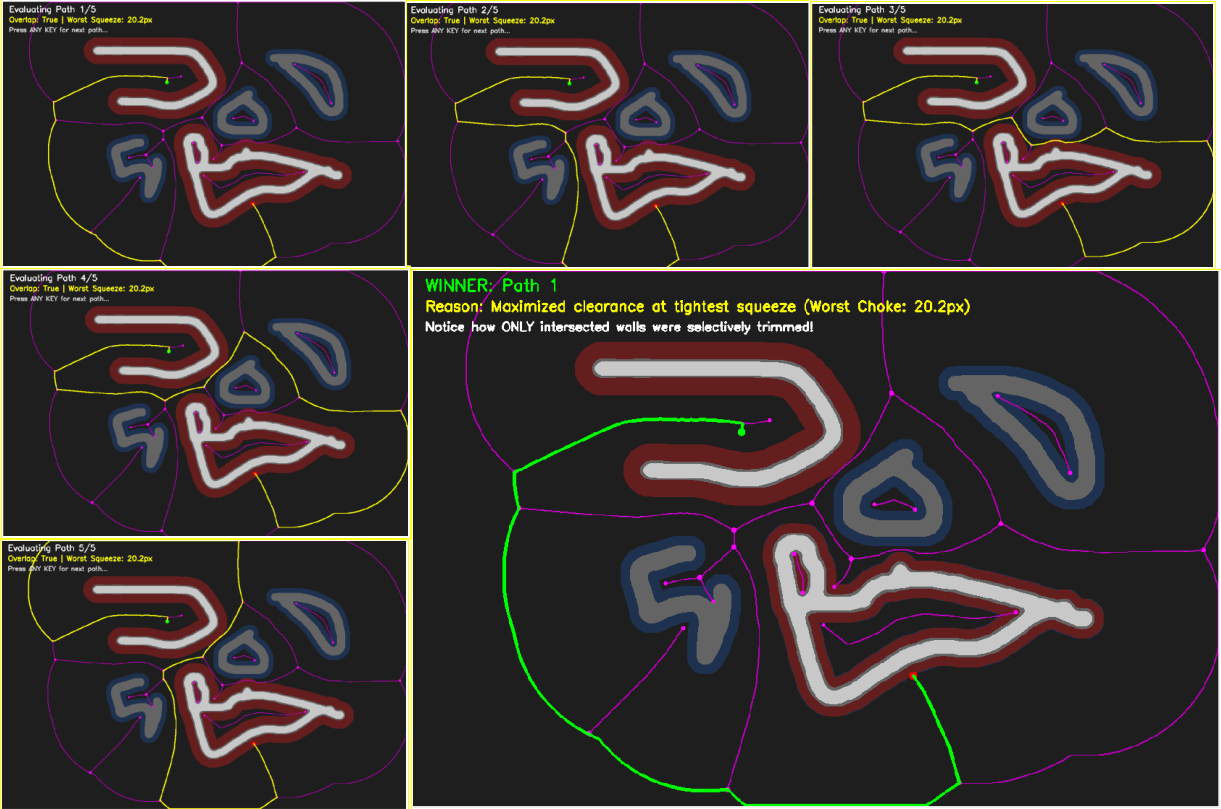
\includegraphics[width=0.96\textwidth]{newsafecomp.png}}
\caption{Homotopy enumeration and lexicographic selection. Panels show $K$ topologically distinct candidates obtained from both injection branches; per-panel annotations give the sorted clearance profile head $(\Psi_{(1)},\Psi_{(2)},\dots)$. The selected route (bottom right) maximizes the tightest passage first and the second-tightest next, which is why it is preferred over the geometrically shorter alternatives. \emph{Reader takeaway: selection is by safety profile, not by length, and the ordering is deterministic.}}
\label{fig:lexicographical}
\end{figure*}

\subsection{Selective Clearance Relaxation}

A uniform repulsion threshold makes the band unable to enter a passage narrower than that threshold: repulsion from both walls dominates contraction and the band stalls or oscillates. Rather than lowering the threshold globally, we lower it only where the selected route requires it.

We label obstacle components by connected-component analysis, obtaining $\{O_1,\dots,O_m\}$ each with its own distance field $\Psi_{O}$. For each component $O$ intersected by $P^\star$ we record the tightest squeeze,
\begin{equation}
s_O=\min_{p\in P^\star}\Psi_O(p),
\end{equation}
and set that component's repulsion threshold to
\begin{equation}
\tau_O=\min\big(\tau_O^{\mathrm{nom}},\ \max(s_O-\eta,\ \rho+\delta_{\mathrm{safe}})\big),
\label{eq:relax}
\end{equation}
where $\tau_O^{\mathrm{nom}}$ is the class-dependent nominal threshold and $\eta$ a small margin. Components not on the route keep $\tau_O^{\mathrm{nom}}$. The clamp at $\rho+\delta_{\mathrm{safe}}$ preserves the safety guarantee: relaxation never goes below the robot radius plus margin, and a passage requiring more relaxation than this is declined rather than executed (Sec.~\ref{sec:setup}). Eq.~\eqref{eq:relax} is evaluated once per query, before tensioning. Removing it (Table~\ref{tab:kinematics}) raises integrated curvature by $37.6\%$ and drops the settled fraction from $83.8\%$ to $67.5\%$.

\subsection{Damped Spring--Mass Band}

Discretize $P^\star$ into nodes $\{P_i\}_{i=1}^{N}$ with $P_1,P_N$ fixed. Node dynamics are
\begin{equation}
\ddot{P}_i = W_s \vec{F}^{\,s}_i + W_r \vec{F}^{\,r}_i - D\,\dot{P}_i ,
\label{eq:dyn}
\end{equation}
with a Hookean contraction term carrying an explicit rest length,
\begin{equation}
\vec{F}^{\,s}_i=\!\!\sum_{j\in\{i-1,i+1\}}\!\!\frac{P_j-P_i}{\|P_j-P_i\|}\Big(\|P_j-P_i\|-d_{\mathrm{rest}}\Big),
\end{equation}
and a per-component repulsion term active only inside the relaxed threshold,
\begin{equation}
\vec{F}^{\,r}_i=\sum_{O}\ \frac{\nabla\Psi_O(P_i)}{\|\nabla\Psi_O(P_i)\|}\ \big[\tau_O-\Psi_O(P_i)\big]_+ ,
\end{equation}
where $[\cdot]_+=\max(\cdot,0)$, so a node outside the threshold feels no force from that component.

The rest length $d_{\mathrm{rest}}$ targets node clumping: a classical elastic band without it admits any node distribution along the curve as an equilibrium, so nodes drift and bunch. With $d_{\mathrm{rest}}$, uniform spacing is the unique equilibrium of the contraction term, and the measured spacing dispersion falls from $0.153$ to $0.101$ (Table~\ref{tab:kinematics}). The damping term $-D\dot{P}_i$ removes the energy that causes sustained oscillation between opposing walls; without it \eqref{eq:dyn} is conservative, and the measured consequence is severe --- integrated curvature rises by a factor of $39$ and only $2.5\%$ of runs settle.

Integration is semi-implicit Euler with time step $h$:
\begin{equation}
\dot{P}_i^{k+1}=\dot{P}_i^{k}+h\,\ddot{P}_i^{k},\qquad P_i^{k+1}=P_i^{k}+h\,\dot{P}_i^{k+1}.
\end{equation}
Node positions are clamped to $\Psi(P_i)\ge\rho+\delta_{\mathrm{safe}}$ after each update, so intermediate iterates are never in collision even before convergence.

\textbf{Distributed decimation.} Slack accumulates as loops that contraction alone shortens slowly. Every $T_{\mathrm{pop}}$ iterations we delete every $N_{\mathrm{pop}}$-th node \emph{uniformly along the whole band} and re-index. Deleting from the ends instead tightens only terminal segments and leaves mid-path loops intact; measured spacing dispersion is $0.101$ for distributed against $0.174$ for end decimation, at equal curvature.

\textbf{Stopping rule.} We track $v^k_{\max}=\max_i\|\dot{P}^k_i\|$ and stop when
\begin{equation}
v^k_{\max}<\epsilon_{\mathrm{stab}}\quad\text{for}\quad n_{\mathrm{hold}}\ \text{consecutive iterations},
\end{equation}
or when an iteration cap is reached. The rule triggered before the cap in $83.8\%$ of runs at $389\pm419$ iterations. Per-iteration cost is $O(N\cdot m_{\mathrm{active}})$ with $m_{\mathrm{active}}$ the number of obstacle components within threshold, typically $\le 3$.

\begin{figure}[htbp]
\centerline{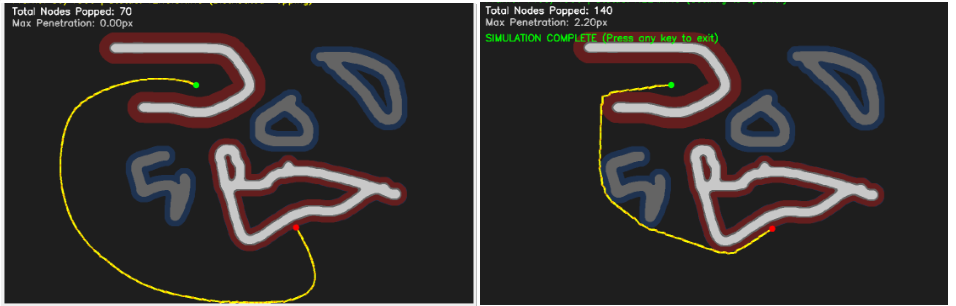
\includegraphics[width=\columnwidth]{rope.png}}
\caption{Band optimization. Left: the selected skeletal route, clearance-maximal but jagged. Right: the settled band after damped tensioning with distributed decimation; the band rests against the selectively relaxed thresholds at the two bottlenecks instead of being repelled out of them. Node markers show that spacing remains uniform. \emph{Reader takeaway: relaxation is applied per obstacle and only where the route demands it, so smoothing does not trade away clearance elsewhere.}}
\label{fig:rope_tensioner}
\end{figure}

\begin{algorithm}[htbp]
\caption{Topological Cage query}
\label{alg:query}
\begin{algorithmic}[1]
\STATE \textbf{Offline (once per map):} $\Psi\!\leftarrow\!\mathrm{EDT}(\Omega)$; $\mathcal{M}\!\leftarrow\!\mathrm{ridge}(\Psi)$
\STATE $\mathcal{M}_{\mathrm{int}}\!\leftarrow\!$ prune by Eq.~\eqref{eq:prune}; $C_{\max}\!\leftarrow\!\sup\Psi$ on $\mathcal{M}_{\mathrm{int}}$
\STATE $\mathcal{C}\!\leftarrow\!\mathcal{M}_{\mathrm{trim}}\cup\{\Psi\!=\!C_{\max}\!+\!\Delta\}$; $G\!\leftarrow\!\mathrm{abstract}(\mathcal{C})$
\STATE \textbf{Online:} \textbf{for} $x\in\{p_S,p_G\}$: integrate Eq.~\eqref{eq:scout} in $\pm$ until $\mathcal{C}$ hit; insert contacts into $G$
\STATE $\{P_1..P_K\}\leftarrow\mathrm{Yen}(G,p_S',p_G',K)$
\STATE $P^\star\leftarrow$ lexicographic max of $\sigma(P_k)$ \hfill (Eq.~\eqref{eq:lex})
\STATE $\{\tau_O\}\leftarrow$ selective relaxation on $P^\star$ \hfill (Eq.~\eqref{eq:relax})
\STATE \textbf{if} any $\tau_O$ clamped at floor for all candidates \textbf{then return} unresolved
\STATE iterate Eq.~\eqref{eq:dyn} with decimation until $v_{\max}<\epsilon_{\mathrm{stab}}$
\STATE \textbf{return} settled band
\end{algorithmic}
\end{algorithm}

% ==========================================
% VII. IMPLEMENTATION AND PARAMETERS
% ==========================================
\section{Implementation and Parameters}
\label{sec:impl}

The system is implemented in Python with NumPy, OpenCV and NetworkX, using an exact Euclidean distance transform~\cite{felzenszwalb2012} and Yen's $K$-shortest-path routine~\cite{yen1971}. All stages run single-threaded. Parameters are held fixed across every environment and every reported run; their values are listed in Table~\ref{tab:params}, and Sec.~\ref{sec:ablation} sweeps the four that admit meaningful ranges.

\begin{table}[htbp]
\caption{Parameters used in all reported experiments}
\label{tab:params}
\begin{center}
\begin{tabular}{@{}llll@{}}
\toprule
\textbf{Param} & \textbf{Value} & \textbf{Param} & \textbf{Value} \\ \midrule
$\tau$ & $17^\circ$ & $W_s$ & $0.55$ \\
$\Delta$ & $20$ px & $W_r$ & $2.50$ \\
$\alpha$ & $0.5$ px & $D$ & $0.40$ \\
$K$ & $5$ & $h$ & $1.0$ \\
$d_{\mathrm{rest}}$ & $5.0$ px & $\epsilon_{\mathrm{stab}}$ & $0.7$ px/iter \\
init.\ spacing & $8.0$ px & $n_{\mathrm{hold}}$ & $30$ \\
$\rho+\delta_{\mathrm{safe}}$ & $6$ px ($0.12$ m) & $N_{\mathrm{pop}},T_{\mathrm{pop}}$ & $10,\,20$ \\
$\tau^{\mathrm{nom}}_{\mathrm{rigid}}$ & $30$ px & $\tau^{\mathrm{nom}}_{\mathrm{soft}}$ & $15$ px \\
$\eta$ & $2.0$ px & iter.\ cap & $1500$ \\
grid res.\ $r$ & $0.02$ m/px & max.\ overlap & $0.85$ \\ \bottomrule
\end{tabular}
\end{center}
\end{table}

% ==========================================
% VIII. EXPERIMENTAL SETUP
% ==========================================
\section{Experimental Setup}
\label{sec:setup}

\textbf{Benchmark suite.} Four maps, each $500\times750$ px at $0.02$ m/px ($10.0\times15.0$ m, $150$ m$^2$), used for all quantitative claims. \textbf{E1}: structured indoor layout with rooms, doorways and soft furniture. \textbf{E2}: semi-sparse map with a large open region, the Voronoi-void stress case. \textbf{E3}: five free-standing obstacle islands with no continuous interior walls. \textbf{E4}: U-shaped non-convex trap with a single $22$-px exit corridor. Obstacles carry semantic class labels (rigid / deformable) with distinct nominal clearance thresholds.

\textbf{Complex operator-drawn maps.} Three additional environments were drawn by an operator at substantially higher geometric complexity than the benchmark suite --- nested spiral corridors with mixed semantic boundaries, five free-standing islands with concave cavities, and a dense multi-branch maze. These match the E1, E3 and E4 topology classes respectively and are used as qualitative case studies (Sec.~\ref{sec:casestudy}); the E2 topology class is covered by the Voronoi-void study in Appendix~\ref{appendix:voronoi_void}.

\textbf{Resolution criterion.} A query is \emph{resolved} if at least one of the $K$ enumerated candidates admits a band solution whose per-component relaxed thresholds all remain above the hard floor $\rho+\delta_{\mathrm{safe}}$ of Eq.~\eqref{eq:relax}. If every candidate would require relaxation below that floor --- i.e.\ the only available passages are narrower than the robot plus its safety margin --- the query is reported as \emph{unresolved} rather than executed. This is a deliberate refusal to traverse an unsafe gap, not a search failure. The criterion is monotone in $K$: enlarging the enumeration budget can convert unresolved queries to resolved but never the reverse. All baselines are scored against the same clearance floor.

\textbf{Baselines.} A$^\star$ on the metric grid~\cite{hart1968}; PRM with $2500$ samples and $k=12$, density tuned to capture the narrowest doorway~\cite{kavraki1996}; RRT$^\star$~\cite{karaman2011} with goal bias $0.05$; GVD routing with A$^\star$-based terminal connection (the injection baseline); EGVG-style contour augmentation with raycast terminal connection~\cite{qi2025egvg}; and a myopic DWA-style local planner~\cite{fox1997} for the trap study. A$^\star$ additionally serves as the reachability oracle: a start--goal pair is \emph{attainable} if A$^\star$ solves it, which normalizes feasibility against the connectivity of the free space itself.

\textbf{Metrics.} Connected components of the routing structure before and after closure; query feasibility, raw and normalized by attainability; injection success and connector-collision rate; minimum and mean path clearance; path length; integrated absolute curvature $\int|\kappa|\,ds$ and angular jerk (RMS third difference of heading); node-spacing coefficient of variation; settling iterations; offline and per-query time split into injection / enumeration / selection / tensioning; graph $|V|,|E|$.

\textbf{Protocol.} $Q=100$ randomized start--goal pairs per environment ($400$ total), sampled uniformly over free cells with $\Psi>\rho+\delta_{\mathrm{safe}}$ and separated by at least $120$ px, with identical pairs across all methods. Injection statistics use $200$ additional randomized terminals per environment ($800$ total). Band ablations use $40$ queries per environment ($160$ total per variant). Selection statistics are restricted to the $375$ queries yielding at least two distinct candidates. All planning runs single-threaded on \PH{CPU model, RAM}.

% ==========================================
% IX. RESULTS
% ==========================================
\section{Results}
\label{sec:results}

\subsection{Closure and Global Connectivity}
\label{sec:res-connectivity}

Table~\ref{tab:connectivity} isolates the effect of closure, and it is the central result of the paper. Summed over the four maps the raw pruned skeleton splits into $21$ components; after adding the level set $\mathcal{B}$ this falls to $5$, and E2--E4 collapse to a single component each. The consequence for planning is direct: feasibility rises from $24.0\%$ to $92.8\%$ raw, and from $25.9\%$ to $99.6\%$ once normalized by attainability.

The effect is largest exactly where the theory predicts. In the open-room map E2 the uncaged planner resolves $7\%$ of queries and the caged planner resolves every attainable one; in the island map E3 the figures are $13\%$ and $100\%$. E1 is the one map whose free space is itself partitioned by sealed room walls, capping any planner at $72\%$; the cage reaches $71$ of those $72$, or $98.6\%$ of attainable. Across all four maps the caged planner leaves a single attainable query unresolved.

\begin{table}[htbp]
\caption{Effect of closure on connectivity and query feasibility}
\label{tab:connectivity}
\begin{center}
\begin{tabular}{@{}lcccccc@{}}
\toprule
\textbf{Env} & \textbf{Comp.} & \textbf{Comp.} & \textbf{Attain.} & \textbf{Raw} & \textbf{Caged} & \textbf{Caged} \\
& \textbf{raw} & \textbf{caged} & \textbf{(\%)} & \textbf{(\%)} & \textbf{(\%)} & \textbf{norm.\ (\%)} \\ \midrule
E1 & $8$ & $2$ & $72$ & $25.0$ & $71.0$ & $98.6$ \\
E2 & $4$ & $\mathbf{1}$ & $100$ & $7.0$ & $\mathbf{100.0}$ & $\mathbf{100.0}$ \\
E3 & $6$ & $\mathbf{1}$ & $100$ & $13.0$ & $\mathbf{100.0}$ & $\mathbf{100.0}$ \\
E4 & $3$ & $\mathbf{1}$ & $100$ & $51.0$ & $\mathbf{100.0}$ & $\mathbf{100.0}$ \\ \midrule
Total/Mean & $21$ & $\mathbf{5}$ & $93$ & $24.0$ & $92.8$ & $\mathbf{99.6}$ \\ \bottomrule
\end{tabular}
\end{center}
\footnotesize Attainability is the A$^\star$ solve rate on the same pairs; normalized feasibility is caged feasibility divided by attainability.
\end{table}

\begin{figure}[htbp]
\centerline{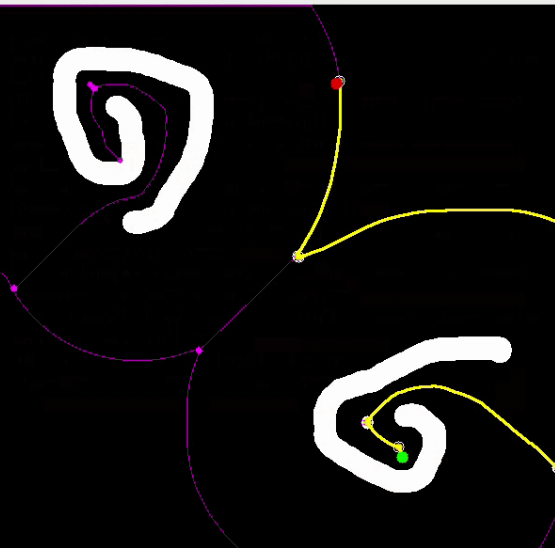
\includegraphics[width=0.85\columnwidth]{isolated_island_navigation.png}}
\caption{Island topology (E3). Free-standing obstacles produce six skeleton components with no mutual connection; the super-critical level set (purple) encloses all of them into one structure, raising feasibility from $13\%$ to $100\%$. \emph{Reader takeaway: closure, not bridging heuristics, is what restores global connectivity.}}
\label{fig:isolated_island}
\end{figure}

\subsection{Search-Free Terminal Injection}
\label{sec:res-injection}

Table~\ref{tab:injection} compares attachment mechanisms over $800$ randomized terminals. Gradient injection is the only mechanism achieving both $100\%$ success and zero connector collisions. Nearest-pixel projection matches the success rate but routes $2.1\%$ of connectors through obstacles, confirming that geometric projection is unsafe. The A$^\star$ fallback is safe and complete but expands $2{,}443$ cells per terminal --- $41.5\times$ our step count --- and is $4.4\times$ slower. Raycast injection is the fastest but drops to $93.5\%$ in E4, where vertex placement leaves terminals without line of sight.

\begin{table}[htbp]
\caption{Injection mechanism comparison (800 randomized terminals)}
\label{tab:injection}
\begin{center}
\begin{tabular}{@{}lcccc@{}}
\toprule
\textbf{Mechanism} & \textbf{Success} & \textbf{Time} & \textbf{Steps /} & \textbf{Collide} \\
& \textbf{(\%)} & \textbf{(ms)} & \textbf{expans.} & \textbf{(\%)} \\ \midrule
Nearest-pixel & $100.0$ & $0.879$ & --- & $2.1$ \\
A$^\star$ to skeleton & $100.0$ & $3.182$ & $2443.3$ & $0.0$ \\
Raycast~\cite{qi2025egvg} & $98.4$ & $\mathbf{0.079}$ & --- & $0.0$ \\
\textbf{Gradient (ours)} & $\mathbf{100.0}$ & $0.727$ & $\mathbf{58.9}$ & $\mathbf{0.0}$ \\ \bottomrule
\end{tabular}
\end{center}
\end{table}

The expansion-count gap is the substantive one. Injection cost is bounded by the clearance span divided by the step size and is independent of map area, whereas the search-based fallback expands cells proportional to the distance from the terminal to the nearest skeleton pixel --- which is largest precisely in the open regions where the skeleton is sparsest. Appendix~\ref{appendix:voronoi_void} reports the measured asymmetry: $3{,}068$ expansions per terminal in the open map E2 against $2{,}031$ in the structured map E1.

\subsection{Complex Environments}
\label{sec:casestudy}

Fig.~\ref{fig:casestudy} shows the full pipeline on the three operator-drawn maps. These exceed the benchmark suite in corridor count, branching factor and boundary curvature: the first contains nested spiral corridors with interleaved rigid and deformable boundaries, the second five free-standing islands with concave cavities and no continuous interior walls, and the third a dense maze whose graph carries substantially more junction vertices than any synthetic map.

In each case the cage unified the skeleton into a single routing manifold, both terminals injected without search, $K=5$ topologically distinct candidates were enumerated, and the lexicographic criterion returned a winner. All three queries resolved under the criterion of Sec.~\ref{sec:setup}. The magenta overlay renders the cage together with the enumerated graph; the green route is the selected class. The selective relaxation of Eq.~\eqref{eq:relax} is directly visible as locally thinned clearance shells on exactly those obstacle components the selected route contacts, while every other component retains its full nominal threshold --- the island map makes this clearest, where the two islands away from the route keep their unthinned red shells.
pipeline
\begin{figure*}[htbp]
\centerline{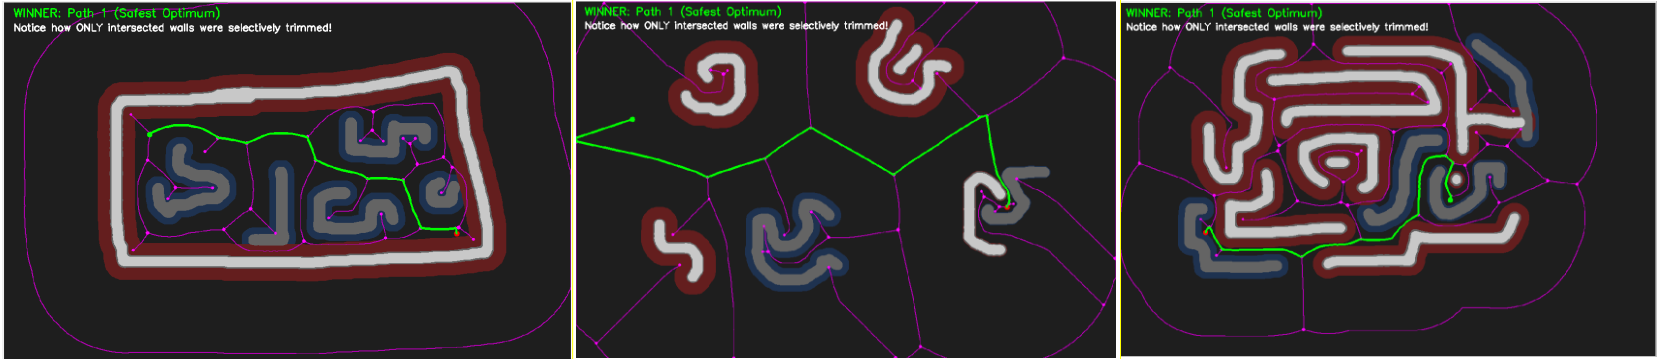
\includegraphics[width=0.98\textwidth]{E134.png}}
\caption{The pipeline on three operator-drawn environments of substantially higher geometric complexity than the benchmark suite. Left: nested spiral corridors with mixed rigid (grey/red) and deformable (blue) semantic boundaries. Centre: five free-standing islands with concave cavities. Right: dense multi-branch maze. In all three, the cage (magenta) unifies the skeleton into a single routing manifold, both terminals inject without grid expansion, $K=5$ distinct homotopy classes are enumerated, and the lexicographic criterion selects the green route. Clearance shells are thinned only on the obstacle components the selected route actually contacts; components away from the route retain their nominal thresholds. \emph{Reader takeaway: enumeration, selection and per-component relaxation behave as specified under geometric complexity well beyond the benchmark suite.}}
\label{fig:casestudy}
\end{figure*}

\subsection{Clearance and Homotopy Selection}
\label{sec:res-selection}

Table~\ref{tab:clearance} compares selection criteria over $375$ multi-candidate queries. The lexicographic order and max-min-clearance agree exactly on minimum clearance ($1.001$~m), as the theory requires, and both improve on shortest-length selection by $3.0\%$. The refinement shows up where it should: ties fall from $247$ to $107$, a $56.7\%$ reduction, and mean clearance along the whole route rises from $1.557$~m to $1.588$~m. The price is $7.3\%$ additional path length over the shortest candidate, which is the cost the criterion is designed to accept.

\begin{table}[htbp]
\caption{Path quality by selection criterion (375 multi-candidate queries)}
\label{tab:clearance}
\begin{center}
\begin{tabular}{@{}lcccc@{}}
\toprule
\textbf{Criterion} & \textbf{Min clr} & \textbf{Mean clr} & \textbf{Len} & \textbf{Ties} \\
& \textbf{(m)} & \textbf{(m)} & \textbf{(m)} & \\ \midrule
Shortest length & $0.972$ & $1.530$ & $\mathbf{10.78}$ & $1$ \\
Max min-clearance & $\mathbf{1.001}$ & $1.557$ & $11.10$ & $247$ \\
\textbf{Lexicographic} & $\mathbf{1.001}$ & $\mathbf{1.588}$ & $11.56$ & $\mathbf{107}$ \\ \bottomrule
\end{tabular}
\end{center}
\end{table}

In the E4 trap environment ($33$ trials, start inside the U, goal outside), the myopic local planner was captured in $33/33$ trials, never escaping the concavity. RRT$^\star$ and our pipeline both resolved $33/33$. The distinction is not success but guarantee: our route is selected by clearance profile over enumerated classes, whereas the sampling planner returns whichever class it happens to find, and the maze case study of Table~\ref{tab:maze} shows that class can graze obstacles.

\subsection{Trajectory Quality and Band Behaviour}
\label{sec:res-band}

Table~\ref{tab:kinematics} compares the raw skeletal route against the settled band and its ablations over $160$ queries per variant. Relative to the raw route, the full band reduces integrated absolute curvature by $85.2\%$ ($26.96\rightarrow3.98$), angular jerk by $74.8\%$ ($0.662\rightarrow0.167$), and node-spacing dispersion by $97.4\%$ ($3.810\rightarrow0.101$), while shortening the path by $20.3\%$.

Damping is decisive. Removing it raises curvature by a factor of $39$, inflates path length from $11.04$~m to $85.49$~m as the band flails between opposing walls, and leaves only $2.5\%$ of runs settled within the iteration cap. Selective relaxation contributes a $37.6\%$ curvature reduction and raises the settled fraction from $67.5\%$ to $83.8\%$. Distributed decimation halves spacing dispersion relative to end decimation ($0.101$ vs $0.174$) at equal curvature. The auto-stop rule triggered before the cap in $83.8\%$ of runs, at $389\pm419$ iterations.

The rest-length term acts specifically and only on spacing uniformity, reducing dispersion from $0.153$ to $0.101$; it does not improve curvature, and we scope the claim accordingly.

\begin{table}[htbp]
\caption{Trajectory quality and band ablation (160 queries per variant)}
\label{tab:kinematics}
\begin{center}
\begin{tabular}{@{}lccccc@{}}
\toprule
\textbf{Variant} & $\int|\kappa|ds$ & \textbf{Jerk} & \textbf{CV} & \textbf{Min clr} & \textbf{Settled} \\
& & & & \textbf{(m)} & \textbf{(\%)} \\ \midrule
Raw skeletal & $26.96$ & $0.662$ & $3.810$ & $0.814$ & --- \\
No damping & $155.11$ & $1.084$ & $0.648$ & $0.347$ & $2.5$ \\
No relaxation & $5.48$ & $0.219$ & $0.185$ & $0.619$ & $67.5$ \\
End decimation & $3.94$ & $0.147$ & $0.174$ & $0.606$ & $\mathbf{86.9}$ \\
\textbf{Full} & $3.98$ & $0.167$ & $\mathbf{0.101}$ & $0.589$ & $83.8$ \\
No rest length & $\mathbf{2.77}$ & $\mathbf{0.121}$ & $0.153$ & $0.602$ & $70.6$ \\ \bottomrule
\end{tabular}
\end{center}
\end{table}

\textbf{Hardware validation.} Physical trials on a differential-drive TurtleBot~3 under overhead motion capture with floor projection of the cage, scouts and live band are \PH{in progress; N trials per environment}. All results above are planner-side geometric measurements.

\subsection{Computational Cost}
\label{sec:res-cost}

Table~\ref{tab:compute_benchmarks} reports the cost of $100$ consecutive randomized queries averaged over the four environments. A$^\star$ pays a full expansion per query, averaging $44{,}345$ cells and $250.2$~ms. Our global routing stage --- injection, enumeration and selection --- costs $24.7$~ms, a $10.1\times$ reduction, against a one-time offline cost of $343.9$~ms. Break-even therefore occurs after $2$ queries, and over $100$ queries the total falls from $25.02$~s to $2.81$~s.

Two baselines are faster in raw wall time but pay for it in feasibility. GVD with A$^\star$ terminal connection completes queries in $17.4$~ms but resolves only $33.5\%$, because its skeleton is disconnected. EGVG-style raycast injection is the fastest attachment mechanism at $0.5$~ms but reaches $90.0\%$. Our method is the only entry matching the attainability ceiling.

The full pipeline including band optimization costs $84.7\pm60.2$~ms. Both rows are reported because the smoothing stage produces an executable trajectory that none of the baselines generate; the $24.7$~ms row is the like-for-like global-routing comparison.

\begin{table}[htbp]
\caption{Cost over 100 consecutive queries, averaged over E1--E4}
\label{tab:compute_benchmarks}
\begin{center}
\begin{tabular}{@{}lcccc@{}}
\toprule
\textbf{Method} & \textbf{Offline} & \textbf{Query} & \textbf{Total} & \textbf{Resolved} \\
& (ms) & (ms) & (s) & (\%) \\ \midrule
A$^\star$ & $0.0$ & $250.2$ & $25.02$ & $93.0$ \\
RRT$^\star$ & $0.0$ & $117.6$ & $11.76$ & $92.5$ \\
PRM (dense) & $945.5$ & $8.2$ & $1.77$ & $84.3$ \\
GVD + A$^\star$ inject & $114.7$ & $17.4$ & $1.85$ & $33.5$ \\
EGVG-style~\cite{qi2025egvg} & $343.9$ & $0.5$ & $0.39$ & $90.0$ \\ \midrule
\textbf{Ours} (routing) & $\mathbf{343.9}$ & $\mathbf{24.7}$ & $\mathbf{2.81}$ & $\mathbf{92.8}$ \\
\textbf{Ours} (+ band) & $343.9$ & $84.7$ & $8.81$ & $92.8$ \\ \bottomrule
\end{tabular}
\end{center}
\end{table}

\begin{table}[htbp]
\caption{Per-query breakdown and graph size}
\label{tab:breakdown}
\begin{center}
\begin{tabular}{@{}lccccc@{}}
\toprule
\textbf{Env} & \textbf{Inject} & \textbf{Enum} & \textbf{Select} & \textbf{Tension} & \textbf{$|V|/|E|$} \\
& (ms) & (ms) & (ms) & (ms) & \\ \midrule
E1 & $1.49$ & $30.83$ & $0.31$ & $63.78$ & $115/161$ \\
E2 & $4.43$ & $15.97$ & $0.42$ & $45.86$ & $52/75$ \\
E3 & $1.60$ & $28.01$ & $0.33$ & $42.71$ & $75/114$ \\
E4 & $1.12$ & $13.71$ & $0.46$ & $61.93$ & $45/63$ \\ \midrule
Mean & $2.16$ & $22.13$ & $0.38$ & $53.57$ & $72/103$ \\ \bottomrule
\end{tabular}
\end{center}
\end{table}

The breakdown locates the cost precisely. Injection is $2.16$~ms and selection $0.38$~ms; enumeration at $22.13$~ms dominates the routing stage, and the $K$-sweep of Sec.~\ref{sec:ablation} shows clearance saturates at $K=3$, so this is reducible without loss. Graph sizes of $45$--$115$ vertices on $375{,}000$-pixel maps confirm that $|V|$ tracks topology rather than area.

An independent single-query maze benchmark on a separate map (Table~\ref{tab:maze}) corroborates the expansion-count argument at the extreme: our method visits $98$ nodes where A$^\star$ visits $244{,}021$ and FMM $360{,}000$, while attaining the highest clearance of any method tested and being the only skeleton-free method to both succeed and stay off the obstacle boundary.

\begin{table}[htbp]
\caption{Single-query maze case study (separate map; clearance in pixels)}
\label{tab:maze}
\begin{center}
\begin{tabular}{@{}lcccc@{}}
\toprule
\textbf{Algorithm} & \textbf{Nodes} & \textbf{Clear.} & \textbf{Time} & \textbf{Success} \\
& \textbf{visited} & \textbf{(px)} & \textbf{(ms)} & \\ \midrule
A$^\star$ & $244{,}021$ & $1.0$ & $3695.99$ & yes \\
PRM & $1{,}002$ & $3.0$ & $430.76$ & yes \\
RRT$^\star$ & $1{,}191$ & $0.0$ & $473.77$ & no \\
FMM & $360{,}000$ & $0.0$ & $176.22$ & no \\
\textbf{Ours} & $\mathbf{98}$ & $\mathbf{14.0}$ & $\mathbf{28.38}$ & \textbf{yes} \\ \bottomrule
\end{tabular}
\end{center}
\end{table}

% ==========================================
% X. ABLATIONS
% ==========================================
\section{Ablation Studies}
\label{sec:ablation}

Each ablation targets one claim. A2 is reported in Table~\ref{tab:injection}, A4 in Table~\ref{tab:clearance}, and A5 in Table~\ref{tab:kinematics}; A1, A3 and A6 follow here.

\textbf{A1 --- Closure.} Removing $\mathcal{B}$ and routing on $\mathcal{M}_{\mathrm{trim}}$ alone drops feasibility from $94.4\%$ to $25.6\%$ (Table~\ref{tab:ablation}). Closure is necessary, not incidental, and the effect is largest on the island and open-room maps.

\textbf{A3 --- Bidirectional scouts.} The climber branch alone attaches $83.8\%$ of terminals. The bidirectional pair reaches $94.4\%$: the diver contributes $10.6$ percentage points in exactly the configurations where the climber stalls on an open-space clearance plateau before reaching the envelope, which is why both branches are retained.

\textbf{A6 --- Parameter sensitivity.} Table~\ref{tab:sweep} sweeps the four free parameters. Feasibility is invariant at $91.3\%$ across $\tau\in[8^\circ,45^\circ]$ and $\Delta\in[5,80]$~px, with graph size varying by under $9\%$ and mean clearance by under $7\%$. This answers the obvious objection to fixed constants: the construction does not depend on them within any reasonable range. Clearance saturates at $K=3$, so the enumeration budget can be cut without loss. Injection succeeds on $100\%$ of terminals for $\alpha\in[0.25,2.0]$~px with step counts falling from $127.5$ to $17.2$; running at $\alpha=2.0$ would reduce injection cost by a further $3.7\times$ at no measured loss.

\begin{table}[htbp]
\caption{Ablation results (mean over E1--E4)}
\label{tab:ablation}
\begin{center}
\begin{tabular}{@{}llccc@{}}
\toprule
\textbf{ID} & \textbf{Variant} & \textbf{Feas.\ \%} & \textbf{Min clr (m)} & \textbf{Query (ms)} \\ \midrule
A1 & no closure & $25.6$ & $0.907$ & $10.2$ \\
A2a & nearest-pixel & $100.0^{\ast}$ & --- & $0.9$ \\
A2b & A$^\star$ inject & $100.0^{\ast}$ & --- & $3.2$ \\
A2c & raycast inject & $98.4^{\ast}$ & --- & $0.1$ \\
A3 & climber only & $83.8$ & $0.870$ & $26.2$ \\
A3 & climber + diver & $\mathbf{94.4}$ & $0.863$ & $27.9$ \\
A4 & shortest-length & $94.4$ & $0.972$ & $27.9$ \\
A5 & no relaxation & $94.4$ & $0.619$ & $27.9$ \\
-- & \textbf{full} & $\mathbf{94.4}$ & $0.863$ & $27.9$ \\ \bottomrule
\end{tabular}
\end{center}
\footnotesize $^{\ast}$attachment success; see Table~\ref{tab:injection} for collision rates.
\end{table}

\begin{table}[htbp]
\caption{Parameter sensitivity (A6), mean over E1--E4}
\label{tab:sweep}
\begin{center}
\begin{tabular}{@{}lcccc@{}}
\toprule
\textbf{Sweep} & \textbf{Value} & \textbf{Feas.\ \%} & \textbf{$|V|$} & \textbf{Min clr (m)} \\ \midrule
\multirow{6}{*}{$\tau$ (deg)}
& $8$  & $91.3$ & $69.8$ & $0.904$ \\
& $12$ & $91.3$ & $73.3$ & $0.860$ \\
& $17$ & $91.3$ & $72.5$ & $0.864$ \\
& $22$ & $91.3$ & $73.0$ & $0.869$ \\
& $30$ & $91.3$ & $69.5$ & $0.843$ \\
& $45$ & $91.3$ & $67.5$ & $0.840$ \\ \midrule
\multirow{5}{*}{$\Delta$ (px)}
& $5$  & $91.3$ & $71.0$ & $0.891$ \\
& $10$ & $91.3$ & $73.8$ & $0.876$ \\
& $20$ & $91.3$ & $72.5$ & $0.864$ \\
& $40$ & $91.3$ & $69.5$ & $0.852$ \\
& $80$ & $91.3$ & $69.3$ & $0.885$ \\ \midrule
& & & \textbf{Query (ms)} & \\ \cmidrule(l){4-4}
\multirow{5}{*}{$K$}
& $1$  & $91.3$ & $5.9$  & $0.850$ \\
& $3$  & $91.3$ & $25.5$ & $0.864$ \\
& $5$  & $91.3$ & $27.4$ & $0.864$ \\
& $8$  & $91.3$ & $26.9$ & $0.864$ \\
& $12$ & $91.3$ & $27.3$ & $0.864$ \\ \midrule
& & \textbf{Inject \%} & \textbf{Steps} & \\ \cmidrule(l){3-4}
\multirow{5}{*}{$\alpha$ (px)}
& $0.25$ & $100.0$ & $127.5$ & --- \\
& $0.5$  & $100.0$ & $64.5$  & --- \\
& $1.0$  & $100.0$ & $33.0$  & --- \\
& $2.0$  & $100.0$ & $17.2$  & --- \\
& $4.0$  & $87.5$  & $508.0$ & --- \\ \bottomrule
\end{tabular}
\end{center}
\end{table}

% ==========================================
% XI. LIMITATIONS
% ==========================================
\section{Limitations}

\textbf{Narrow-passage refusal.} When every enumerated candidate would require clearance relaxation below $\rho+\delta_{\mathrm{safe}}$, the planner declines rather than executes. This is the intended behaviour --- the passage is genuinely narrower than the robot plus its margin --- but it means no path is returned in configurations where a kinodynamically aggressive planner might squeeze through. The criterion is monotone in $K$, so part of this gap closes with a larger enumeration budget.

\textbf{Static map assumption.} The cage derives from $C_{\max}$, a global statistic. A map change that alters the widest interior corridor changes $d_{\mathrm{cage}}$ and therefore the envelope. Localized changes that do not affect $C_{\max}$ admit local edge repair, but this is not implemented and no timing claims are made for it.

\textbf{Envelope routes carry a length premium.} When the skeleton is genuinely sparse, the selected route may traverse $\mathcal{B}$ around a structure rather than through it. Measured at $7.3\%$ additional length over shortest-candidate selection (Table~\ref{tab:clearance}), this is the cost the lexicographic criterion accepts by design.

\textbf{Enumeration dominates query cost and is not topology-complete.} At $22.1$~ms, Yen enumeration is $10\times$ the injection cost. It samples homotopy classes rather than enumerating them exhaustively, so a class optimal under the clearance order but absent from the $K$ candidates will be missed. Table~\ref{tab:sweep} shows clearance saturates at $K=3$, bounding the practical impact.

\textbf{Feasibility is bounded by free-space connectivity.} The cage cannot connect regions that are genuinely separated, as E1 demonstrates. Closure restores connectivity of the \emph{representation}, not of the workspace.

\textbf{Single global pruning threshold.} $\tau$ does not adapt to local corridor width. Table~\ref{tab:sweep} shows insensitivity over $[8^\circ,45^\circ]$ on these maps, but environments mixing extreme corridor scales may require an adaptive rule.

\textbf{Planar, holonomic output.} The planner produces a 2D geometric path; differential-drive kinematics are handled downstream by pure pursuit, and kinodynamic feasibility is not enforced in the band.

\textbf{Rest-length scope.} The Hookean rest length improves node-spacing uniformity but not curvature; removing it yields marginally smoother paths at $51\%$ higher spacing dispersion. We claim only the spacing effect.

% ==========================================
% XII. CONCLUSION
% ==========================================
\section{Conclusion}

We presented the Topological Cage, a bounded medial manifold built by pruning the medial axis with a tangent--gradient parallelism test and closing it with a distance level set placed above the interior clearance supremum. Closure is what makes the representation usable: it reduces routing-structure components from $21$ to $5$ across four benchmarks and raises query feasibility from $24.0\%$ to $99.6\%$ of attainable, leaving a single attainable query unresolved over $400$. Closure also makes terminal injection a matter of integrating a vector field rather than expanding a frontier, attaching $100\%$ of $800$ randomized terminals with zero connector collisions at $58.9$ steps, against $2{,}443$ expansions for the search-based fallback and $44{,}345$ for full grid search. The resulting cost structure --- one offline construction, queries whose cost tracks topology rather than area --- breaks even against A$^\star$ after two queries and releases budget for enumerating homotopy classes, selected by a lexicographic clearance order that cuts ties by $56.7\%$ while raising mean clearance, and for a damped band that reduces curvature by $85.2\%$ and spacing dispersion by $97.4\%$ while retaining a hard safety floor at $\rho+\delta_{\mathrm{safe}}$. Three operator-drawn environments of substantially higher geometric complexity confirm the behaviour qualitatively, and parameter sweeps show feasibility invariant across wide ranges of $\tau$, $\Delta$, $K$ and $\alpha$, indicating the construction does not rest on tuned constants. The main open direction is incremental cage maintenance under map change, which requires handling the global dependence of $d_{\mathrm{cage}}$ on $C_{\max}$.

% ==========================================
% APPENDIX
% ==========================================
\appendices
\section{The Voronoi Void}
\label{appendix:voronoi_void}

The medial axis is the set of points equidistant to two or more boundary points. In a large open region no such points exist at useful density: the nearest boundaries are far apart and the equidistance locus is sparse or degenerates to a single curve far from any useful corridor. Fig.~\ref{fig:voronoi_problem} shows a query point in such a region with no skeleton within reach. Around a free-standing obstacle the failure differs in kind: the skeleton forms a closed loop \emph{around} the obstacle, a legitimate structure but a separate connected component.

Both failures are measurable. In E2, a semi-sparse map with one large open region, the raw skeleton splits into four components and the resulting planner resolves $7\%$ of randomized queries. In E3, built from five free-standing islands, it splits into six components and resolves $13\%$.

\begin{figure}[htbp]
\centerline{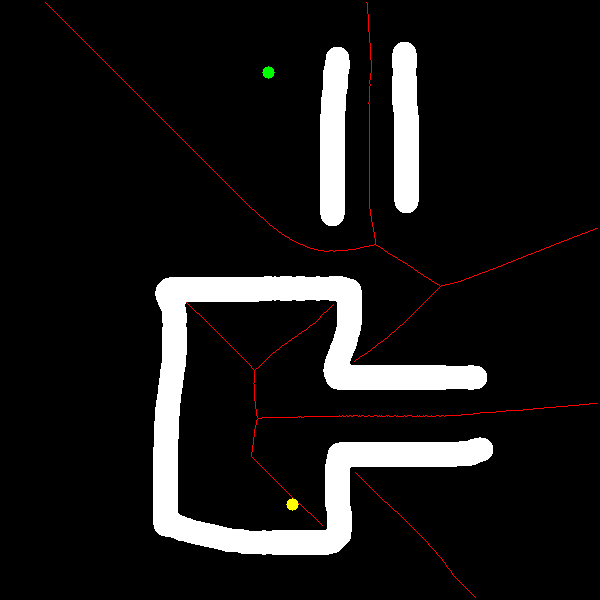
\includegraphics[width=0.85\columnwidth]{voronoi_shortcoming_raw.png}}
\caption{Voronoi void. The standard medial axis (red) provides no structure across the open region, leaving the query point (green) with nothing to connect to. \emph{Reader takeaway: the failure is in the representation, not in the connection procedure.}}
\label{fig:voronoi_problem}
\end{figure}

The standard recourse is a grid search from the query until a skeleton pixel is found, whose cost grows with the size of the void --- precisely the wrong scaling. Our measurements confirm this: the A$^\star$ injection fallback expands $3{,}068$ cells per terminal in E2, the most open of the four maps, against $2{,}031$ in the structured map E1.

The cage removes the need for it. The level set $\mathcal{B}$ passes through the open region by construction, because $\Psi$ attains $d_{\mathrm{cage}}$ there, and gradient ascent reaches that level in arc length at most $d_{\mathrm{cage}}-\Psi(p_0)$. After closure both maps reduce to a single component and resolve every attainable query (Fig.~\ref{fig:voronoi_resolution}).

\begin{figure}[htbp]
\centerline{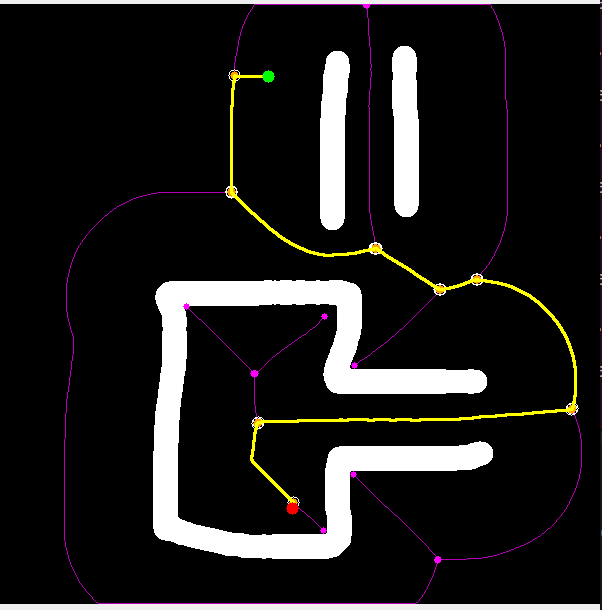
\includegraphics[width=0.85\columnwidth]{voronoi_our_path.png}}
\caption{Resolution by closure. The cage (purple) crosses the open region; the climber reaches it by monotone gradient ascent and the query routes on the unified structure (yellow) with no grid expansion. \emph{Reader takeaway: the envelope supplies routing structure exactly where the medial axis has none.}}
\label{fig:voronoi_resolution}
\end{figure}

% ==========================================
% REFERENCES
% ==========================================
\begin{thebibliography}{00}

\bibitem{qi2025egvg} H. Qi, Y. Zhang, C. Pan, M. Li, F. Meng, Z. Yu, P. Lu, and X. Chen, ``Enveloped Generalized Voronoi Graph and multi-topology path planning for navigation in unknown environments,'' \textit{TechRxiv preprint}, Oct.\ 2025, doi:10.36227/techrxiv.176159300.02637396/v1.

\bibitem{hart1968} P. E. Hart, N. J. Nilsson, and B. Raphael, ``A formal basis for the heuristic determination of minimum cost paths,'' \textit{IEEE Trans. Syst. Sci. Cybern.}, vol. 4, no. 2, pp. 100--107, 1968.

\bibitem{koenig2005} S. Koenig and M. Likhachev, ``Fast replanning for navigation in unknown terrain,'' \textit{IEEE Trans. Robot.}, vol. 21, no. 3, pp. 354--363, 2005.

\bibitem{kavraki1996} L. E. Kavraki, P. \v{S}vestka, J.-C. Latombe, and M. H. Overmars, ``Probabilistic roadmaps for path planning in high-dimensional configuration spaces,'' \textit{IEEE Trans. Robot. Autom.}, vol. 12, no. 4, pp. 566--580, 1996.

\bibitem{lavalle1998} S. M. LaValle, ``Rapidly-exploring random trees: A new tool for path planning,'' Tech. Rep. TR 98-11, Iowa State Univ., 1998.

\bibitem{karaman2011} S. Karaman and E. Frazzoli, ``Sampling-based algorithms for optimal motion planning,'' \textit{Int. J. Robot. Res.}, vol. 30, no. 7, pp. 846--894, 2011.

\bibitem{felzenszwalb2012} P. F. Felzenszwalb and D. P. Huttenlocher, ``Distance transforms of sampled functions,'' \textit{Theory of Computing}, vol. 8, no. 1, pp. 415--428, 2012.

\bibitem{lau2013} B. Lau, C. Sprunk, and W. Burgard, ``Efficient grid-based spatial representations for robot navigation in dynamic environments,'' \textit{Robot. Auton. Syst.}, vol. 61, no. 10, pp. 1116--1130, 2013.

\bibitem{hoff1999} K. E. Hoff III, J. Keyser, M. Lin, D. Manocha, and T. Culver, ``Fast computation of generalized Voronoi diagrams using graphics hardware,'' in \textit{Proc. SIGGRAPH}, 1999, pp. 277--286.

\bibitem{oleynikova2018} H. Oleynikova, Z. Taylor, R. Siegwart, and J. Nieto, ``Sparse 3D topological graphs for micro-aerial vehicle planning,'' in \textit{IEEE/RSJ IROS}, 2018, pp. 1--9.

\bibitem{qi2022pruned} Y. Qi, R. Wang, B. He, F. Lu, and Y. Xu, ``Compact and efficient topological mapping for large-scale environment with pruned Voronoi diagram,'' \textit{Drones}, vol. 6, no. 7, p. 183, 2022.

\bibitem{foskey2003} M. Foskey, M. C. Lin, and D. Manocha, ``Efficient computation of a simplified medial axis,'' in \textit{Proc. ACM Symp. Solid Modeling and Applications}, 2003, pp. 96--107.

\bibitem{chi2022} W. Chi, Z. Ding, J. Wang, G. Chen, and L. Sun, ``A generalized Voronoi diagram-based efficient heuristic path planning method for RRTs in mobile robots,'' \textit{IEEE Trans. Ind. Electron.}, vol. 69, no. 5, pp. 4926--4937, 2022.

\bibitem{zhang2024agv} R. Zhang, R. Chai, S. Chai, Y. Xia, and A. Tsourdos, ``Design and practical implementation of a high efficiency two-layer trajectory planning method for AGV,'' \textit{IEEE Trans. Ind. Electron.}, vol. 71, no. 2, pp. 1811--1822, 2024.

\bibitem{yang2022far} F. Yang, C. Cao, H. Zhu, J. Oh, and J. Zhang, ``FAR planner: Fast, attemptable route planner using dynamic visibility update,'' in \textit{IEEE/RSJ IROS}, 2022, pp. 9--16.

\bibitem{dobson2014} A. Dobson and K. E. Bekris, ``Sparse roadmap spanners for asymptotically near-optimal motion planning,'' \textit{Int. J. Robot. Res.}, vol. 33, no. 1, pp. 18--47, 2014.

\bibitem{quinlan1993} S. Quinlan and O. Khatib, ``Elastic bands: Connecting path planning and control,'' in \textit{IEEE ICRA}, 1993, pp. 802--807.

\bibitem{rosmann2012} C. R\"osmann, W. Feiten, T. W\"osch, F. Hoffmann, and T. Bertram, ``Trajectory modification considering dynamic constraints of autonomous robots,'' in \textit{7th German Conf.\ on Robotics (ROBOTIK)}, 2012, pp. 1--6.

\bibitem{fox1997} D. Fox, W. Burgard, and S. Thrun, ``The dynamic window approach to collision avoidance,'' \textit{IEEE Robot. Autom. Mag.}, vol. 4, no. 1, pp. 23--33, 1997.

\bibitem{yen1971} J. Y. Yen, ``Finding the $k$ shortest loopless paths in a network,'' \textit{Management Science}, vol. 17, no. 11, pp. 712--716, 1971.

\bibitem{bhattacharya2012} S. Bhattacharya, M. Likhachev, and V. Kumar, ``Topological constraints in search-based robot path planning,'' \textit{Autonomous Robots}, vol. 33, no. 3, pp. 273--290, 2012.

\end{thebibliography}

\end{document}

 